\documentclass[11pt,aspectratio=169]{beamer}
\usepackage{minted}
\usepackage{alltt}
\usepackage[utf8]{inputenc}
\usepackage[english]{babel}
\usepackage{xspace}
\usepackage{cancel}

\usetheme[sectionpage=none]{metropolis}
\usepackage[scaled=0.8]{DejaVuSansMono} % A decent mono font
%\usepackage{enumitem}
%\setitemize{noitemsep,topsep=3pt,parsep=3pt,partopsep=3pt}
%\setenumerate{noitemsep,topsep=3pt,parsep=3pt,partopsep=3pt}



\definecolor{green}{rgb}{0, 0.5, 0.1}
\definecolor{magenta}{rgb}{1, 0, 0}


\newcommand{\error}[1]{\textcolor{red}{#1}}
\newcommand{\ok}[1]{\textcolor{green}{#1}}

\title[Functor diffing]{High-level error messages for modules through diffing}
\author[Angeletti \& Radanne]{\texorpdfstring{
  \begin{columns}\column{0.5\linewidth}\centering%
  Florian \textsc{Angeletti}\\
  Inria\\
  \href{mailto:florian.angeletti@inria.fr}
  {\nolinkurl{florian.angeletti@inria.fr}}
  \column{0.5\linewidth}\centering%
  Gabriel \textsc{Radanne}\\
  Inria\\
  \href{mailto:gabriel.radanne@inria.fr}
  {\nolinkurl{gabriel.radanne@inria.fr}}
  \end{columns}
  }{F. Angeletti \& G. Radanne}}
\date{}
\begin{document}
\begin{frame}
\maketitle
\end{frame}

\section{Module errors}

%\begin{frame}
%  \structure{In ML languages, error messages for type error at the module level
%    are notoriously hard to read}.
%\end{frame}

\begin{frame}[fragile,t]\frametitle{}

\begin{minted}{ocaml}
module String_map = Map.Make(String)(String)
\end{minted}
\begin{onlyenv}<2>
\begin{alltt}
\error{Error}: This module is not a functor; it has type
       sig
         type key = String.t
         type 'a t = 'a Map.Make(String).t
         val empty : 'a t
         val is_empty : 'a t -> bool
         val mem : key -> 'a t -> bool
         val add : key -> 'a -> 'a t -> 'a t
         val update : key -> ('a option -> 'a option) -> 'a t -> 'a t
         val singleton : key -> 'a -> 'a t
        \dots(elided for the slide)
       end
\end{alltt}
\end{onlyenv}

\begin{onlyenv}<3>
\begin{alltt}\error{Error}: The functor application is ill-typed.
       These arguments:
         \ok{String} \error{String}
       do not match these parameters:
         functor (Ord : \ok{Map.OrderedType})  -> ...
  \ok{1.} Module String matches the expected module type Map.OrderedType
  \error{2.} The following extra argument is provided
         String : \dots(elided)
\end{alltt}
\end{onlyenv}

\end{frame}


\begin{frame}\frametitle{Modules: theory vs practice}
\begin{description}
\item[Theory:]{Most complex part of the language}
\item[Practice:]{Shallow hierarchy of submodules, a handful of functors with few arguments}
\end{description}

\end{frame}

\begin{frame}[fragile]\frametitle{A typical example}
A common example of functors (such as Ocamlgraph)
\begin{minted}{ocaml}
module Graph(Vertex:VERTEX)(Edge:EDGE) = struct ... end
\end{minted}


\end{frame}

\begin{frame}[fragile]\frametitle{Common errors}

  \begin{itemize}
    \item{Unnecessary argument
\begin{minted}{ocaml}
module G = Graph(Label)(Vertex)(Edge)
\end{minted}
      }
    \item{Forgotten argument:
\begin{minted}{ocaml}
module G = Graph(Edge)
\end{minted}
      }
    \item{Wrong argument:
\begin{minted}{ocaml}
module G = Graph(Label)(Edge)
\end{minted}
      }
\end{itemize}

All those errors are frequent during refactorings.

\end{frame}

\begin{frame}[fragile]
Classical error messages consider only the last alternative:

\begin{minted}{ocaml}
module G = Graph(Label)(Vertex)(Edge)
\end{minted}

\begin{alltt}
\error{Error}: Signature mismatch:
       Modules do not match:
         sig type t = string end
       is not included in
         VERTEX
       The value `label' is required but not provided
       The value `create' is required but not provided
       The type `label' is required but not provided
       The value `equal' is required but not provided
       The value `hash' is required but not provided
       The value `compare' is required but not provided
 \end{alltt}
\end{frame}


\section{Diffing higher level error}


\begin{frame}[fragile]\frametitle{A little bit of perspective}

  For errors, we need to keep the \emph{multi-application} context

Consider the arguments as two lists:
\begin{minted}{ocaml}
 Graph(Label)(Vertex)(Edge)
\end{minted}
\begin{minted}{ocaml}
 module Graph(Vertex:VERTEX)(Edge:EDGE) = ...
\end{minted}

use diffing between lists or strings: addition, deletion, or modification.

\end{frame}

\begin{frame}[fragile]\frametitle{Unnecessary argument}
\begin{minted}{ocaml}
module G=Graph(Label)(Vertex)(Edge)
\end{minted}
\begin{alltt}
{\bfseries{}\color{red}{}Error}: The functor application is ill-typed.
       These arguments:
         {\color{red}{}\bfseries{}Label} {\color{green}{}Vertex} {\color{green}{}Edge}
       do not match these parameters:
         functor {\color{red}{}\bfseries{}} {\color{green}{}(Vertex : VERTEX)} {\color{green}{}(Edge : EDGE)} -> ...
  {\color{red}{}\bfseries{}1.} The following extra argument is provided
      Label : sig type t = string end
  {\color{green}{}2.} Module Vertex matches the expected module type VERTEX
  {\color{green}{}3.} Module Edge matches the expected module type EDGE
\end{alltt}
\end{frame}

\begin{frame}[fragile]\frametitle{Missing argument}
\begin{minted}{ocaml}
module G=Graph(Edge)
\end{minted}
\begin{alltt}
{\bfseries{}\color{red}{}Error}: The functor application is ill-typed.
       These arguments:
         {\color{red}{}\bfseries{}} {\color{green}{}Edge}
       do not match these parameters:
         functor {\color{red}{}\bfseries{}(Vertex : VERTEX)} {\color{green}{}(Edge : EDGE)} -> ...
  {\color{red}{}\bfseries{}1.} An argument appears to be missing with module type VERTEX
  {\color{green}{}2.} Module Edge matches the expected module type EDGE
\end{alltt}
\end{frame}

\begin{frame}[fragile]\frametitle{Wrong argument}
\begin{minted}{ocaml}
module G=Graph(Label)(Edge)
\end{minted}
\begin{alltt}
{\bfseries{}\color{red}{}Error}: The functor application is ill-typed.
       These arguments:
         {\color{magenta}{}\bfseries{}Label} {\color{green}{}Edge}
       do not match these parameters:
         functor {\color{magenta}{}\bfseries{}(Vertex : VERTEX)} {\color{green}{}(Edge : EDGE)} -> ...
  {\color{magenta}{}\bfseries{}1.} Modules do not match:
       Label : sig type t = string end
     is not included in
       VERTEX
     \dots(elided for the slide)
  {\color{green}{}2.} Module Edge matches the expected module type EDGE

\end{alltt}
\end{frame}

\begin{frame}[standout]
  \centering \Huge How does this work?
\end{frame}
\begin{frame}\frametitle{String diffing}
\begin{block}{}
  Error classes seen this far: Addition, Deletion, Change
\end{block}
\begin{block}{}
   Those are classical errors in string diffing
 \end{block}
 \begin{block}{}String diffing is everywhere:
   spellchecking, fuzzy search, control version, DNA sequence matching, ...
 \end{block}

\end{frame}

\begin{frame}\frametitle{String diffing -- details}
  Typical operations:
  \begin{itemize}
    \item \textbf<2->{Addition}: A B \ok{\underline{C}} D
    \item \textbf<2->{Deletion}: A B \error{$\xcancel{C}$} D
    \item \textbf<2->{Change}: A B $\cancelto{\ok{C}}{\error{F}}$ D
    \item Swap: A B $\underset{\leftrightarrow}{C\ D}$
  \end{itemize}
  Well-studied topic:
  \begin{itemize}
    \item many distances: \textbf<3>{Levenstein}, LCS, Hamming, ...
     \item many algorithms: \textbf<3>{Wagner-Fischer}, Myers diff, Hirschberg's algorithm, ...
  \end{itemize}
\end{frame}

\begin{frame}[fragile]\frametitle{Wagner-Fischer illustrated}
   \centering 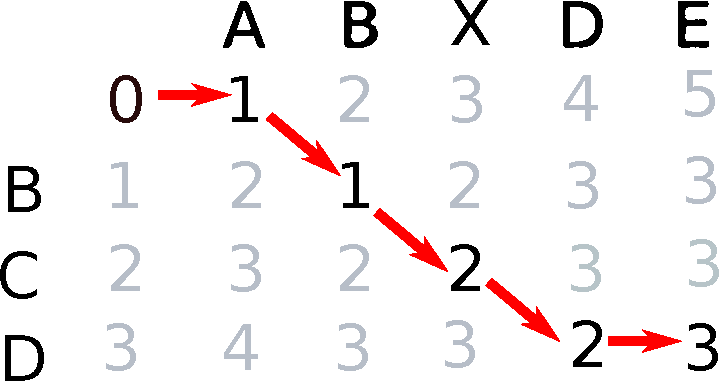
\includegraphics{matrix.pdf}
\end{frame}

\begin{frame}\frametitle{Our choice}
  \structure{Dynamically-sized variant of the Wagner-Fischer algorithm for
    computing distance with addition-deletion-change}
  \begin{itemize}
    \item{Argument comparison: OCaml typechecker comparison used as a black box}
    \item{Complexity: $O(\max(\mathrm{|arguments|,|parameters|})^2)$}
    \item{implemented as a patch on the OCaml compiler:
      \url{https://github.com/ocaml/ocaml/pull/9331} }
  \end{itemize}
\end{frame}


\begin{frame}[fragile]\frametitle{Unreasonably complicated error}
\begin{minted}{ocaml}
module A = Seq module A' = Complex
module B = Option module B' = Bigarray
module C = Result module C' = Bool
module D = Char module D' = Uchar
module E = Sys module E' = List
module F = Bytes module F' = Map.Make
module G = String
\end{minted}
\end{frame}
\begin{frame}[fragile]\frametitle{Unreasonably complicated error}
\begin{minted}{ocaml}
module Little_functor =
    (A: module type of A) (B: module type of B)
    (C: module type of C) (D: module type of D)
    (E: module type of E) (F: module type of F)
    (G: module type of G) (H: module type of H)
    = struct end
\end{minted}
\end{frame}

\begin{frame}[fragile]\frametitle{Unreasonably complicated error}
\begin{minted}{ocaml}
module E = Little_functor(A)(A)(B)(C')(E)(F')(G)(H)(H)
\end{minted}
  \footnotesize
\begin{alltt}
These arguments:
  {\color{green}{}A} {\color{red}{}\bfseries{}A} {\color{green}{}B} {\color{magenta}{}\bfseries{}C'} {\color{red}{}\bfseries{}} {\color{green}{}E} {\color{magenta}{}\bfseries{}F'} {\color{green}{}G} {\color{green}{}H} {\color{red}{}\bfseries{}H'}
do not match these parameters:
  functor {\color{green}{}(A : ...)} {\color{red}{}\bfseries{}} {\color{green}{}(B : ...)} {\color{magenta}{}\bfseries{}(C : ...(C))} {\color{red}{}\bfseries{}(D : ...(D))} {\color{green}{}(E : ...)}
  {\color{magenta}{}\bfseries{}(F : ...(F))} {\color{green}{}(G : ...)} {\color{green}{}(H : ...)} {\color{red}{}\bfseries{}} -> ...
{\color{green}{}1.} Module A matches the expected module type
{\color{red}{}\bfseries{}2.} The following extra argument is provided: \dots(elided)
{\color{green}{}3.} Module B matches the expected module type
{\color{magenta}{}\bfseries{}4.} Modules do not match: C' : \dots(elided)
{\color{red}{}\bfseries{}5.} An argument appears to be missing \dots(elided)
{\color{green}{}6.} Module E matches the expected module type
{\color{magenta}{}\bfseries{}7.} Modules do not match: F' \dots(elided)
{\color{green}{}8.} Module G matches the expected module type
{\color{green}{}9.} Module H matches the expected module type
{\color{red}{}\bfseries{}10.} The following extra argument is provided H' : \dots(elided)
\end{alltt}
\end{frame}



\begin{frame}[fragile]\frametitle{Dependent functors?}
\begin{minted}{ocaml}
module type f =
  functor
    (B:sig type x type y type u=x type v=y end)
    (Y:sig type yu = Y of B.u end)
    (Z:sig type zv = Z of B.v end)
   -> sig end
module F: f =
  functor
    (X:sig type x type y end)
    (Z:sig type zv = Z of X.y end)
   -> struct end
\end{minted}
\end{frame}

\begin{frame}[fragile]\frametitle{Dependent functors?}
\begin{alltt}
{\bfseries{}\color{red}{}Error}: Signature mismatch:
       Modules do not match:
         functor {\color{green}{}(X : ...(X))} {\color{red}{}\bfseries{}} {\color{green}{}(Z : ...(Z))} -> ...
       is not included in
         functor {\color{green}{}(B : ...(B))} {\color{red}{}\bfseries{}(Y : ...(Y))} {\color{green}{}(Z : ...(Z))} -> ...
  {\color{green}{}1.} Module types ...(X) and ...(B) match
  {\color{red}{}\bfseries{}2.} An argument appears to be missing with module type
         ...(Y) = sig type yu = Y of B.u end
  {\color{green}{}3.} Module types ...(Z) and ...(Z) match
\end{alltt}
\end{frame}

\begin{frame}[fragile]\frametitle{Dynamically-sized?}
  Functors are complicated, they can be variadic in OCaml:
   \begin{minted}{ocaml}
 module F(X:sig
   module type t
   module M:t
 end) = X.M
 module Ft = struct
   module M = F
   module type t = module type of F
 end
\end{minted}

\begin{minted}{ocaml}
F(Ft)(Ft)(Ft)(Ft)...
\end{minted}

  Our modified Wagner-Fischer algorithm handles those cases (and yet always terminates).
\end{frame}

\begin{frame}[fragile]\frametitle{What about swaps?}
  Hard to present well in text output.

  We may consider a subcase where all arguments are here:
\begin{minted}{ocaml}
  Graph(Edge)(Vertex)
\end{minted}
\end{frame}



\section{Complex examples}

\begin{frame}[standout]
  \centering \Huge Does this scale?
\end{frame}


\begin{frame}[fragile] \frametitle{A question of performances?}
  \begin{itemize}
    \item{Quadratic module comparisons}
    \item{Errors are for human. Human are slow.}
    \item{Which effect matters?}
  \end{itemize}
\end{frame}

\begin{frame}[fragile]\frametitle{A not that small functor}
  \begin{itemize}
    \item A 26 argument functor, with all stdlib modules involved
  \end{itemize}
\begin{alltt}
These arguments:
  {\color{green}{}A} {\color{red}{}\bfseries{}A} {\color{green}{}B} {\color{magenta}{}\bfseries{}C'} {\color{red}{}\bfseries{}} {\color{green}{}E} {\color{magenta}{}\bfseries{}F'} {\color{green}{}G} {\color{green}{}H} {\color{red}{}\bfseries{}H'} {\color{green}{}I} {\color{green}{}J} {\color{red}{}\bfseries{}} {\color{green}{}L} {\color{green}{}M} {\color{magenta}{}\bfseries{}N'} {\color{green}{}O} {\color{red}{}\bfseries{}O'} {\color{green}{}P} {\color{red}{}\bfseries{}} {\color{green}{}R} {\color{green}{}S} {\color{magenta}{}\bfseries{}T'} {\color{magenta}{}\bfseries{}U'} {\color{green}{}V} {\color{green}{}W} {\color{red}{}\bfseries{}W} {\color{green}{}X} {\color{green}{}Y} {\color{green}{}Z} {\color{red}{}\bfseries{}Z}
do not match these parameters:
  functor {\color{green}{}(A : ...)} {\color{red}{}\bfseries{}} {\color{green}{}(B : ...)} {\color{magenta}{}\bfseries{}(C : ...(C))} {\color{red}{}\bfseries{}(D : ...(D))} {\color{green}{}(E : ...)}
  {\color{magenta}{}\bfseries{}(F : ...(F))} {\color{green}{}(G : ...)} {\color{green}{}(H : ...)} {\color{red}{}\bfseries{}} {\color{green}{}(I : ...)} {\color{green}{}(J : ...)} {\color{red}{}\bfseries{}(K : ...(K))}
  {\color{green}{}(L : ...)} {\color{green}{}(M : ...)} {\color{magenta}{}\bfseries{}(N : ...(N))} {\color{green}{}(O : ...)} {\color{red}{}\bfseries{}} {\color{green}{}(P : ...)} {\color{red}{}\bfseries{}(Q : ...(Q))}
  {\color{green}{}(R : ...)} {\color{green}{}(S : ...)} {\color{magenta}{}\bfseries{}(T : ...(T))} {\color{magenta}{}\bfseries{}(U : ...(U))} {\color{green}{}(V : ...)} {\color{green}{}(W : ...)} {\color{red}{}\bfseries{}}
  {\color{green}{}(X : ...)} {\color{green}{}(Y : ...)} {\color{green}{}(Z : ...)} {\color{red}{}\bfseries{}} -> ...
\end{alltt}

  \begin{itemize}
    \item 100 ms with ocamlopt
  \end{itemize}

\end{frame}


  \begin{frame}[fragile]
  \begin{minted}{ocaml}
module M = F
    (Ft)(Ft)(List)(Ft)(Ft)(Ft)(List)(Ft)(Ft)(List)
    (Ft)(Ft)(Ft)(Ft)(Ft)(Ft)(Ft)(Ft)(Ft)(Ft)(Ft)(Ft)(Ft)
    (Ft)(Ft)(Ft)(Ft)(Ft)(Ft)(Ft)(Ft)(Ft)(Ft)(Ft)(Ft)(Ft)
    (Ft)(Ft)(Ft)(Ft)(Ft)(Arg)(Ft)(Ft)(Ft)(Ft)(Ft)(Ft)(Ft)
    (Ft)(Ft)(Ft)(Ft)(Ft)(Ft)(Ft)(Ft)(Ft)(Ft)(Ft)(Ft)(Ft)
    (Ft)(Ft)(Ft)(Float)(Ft)(Ft)(Ft)(Ft)(Ft)(Ft)(Ft)(Ft)(Ft)
    (Ft)(Ft)(Ft)(Ft)(Ft)(Ft)(Ft)(Ft)(Ft)(Ft)(Ft)(Ft)(Ft)
    (Ft)(Ft)(Ft)(Ft)(Ft)(Gc)(Ft)(Ft)(Ft)(Ft)(Ft)(Ft)(Ft)
    (Ft)(Ft)(Ft)(Ft)(Ft)(Ft)(Ft)(Ft)(Ft)(Ft)(Ft)(Ft)(Ft)
    (Ft)(Ft)(Ft)(Ft)(Ft)(Ft)(Map)(Ft)(Ft)(Ft)(Ft)(Ft)(Ft)
    (Ft)(Ft)(Ft)(Ft)(Ft)(Ft)(Ft)(Ft)(Ft)(Ft)(Ft)(Ft)(Ft)
    (Ft)(Ft)(Seq)(Ft)(Ft)(Ft)(Ft)(Ft)(Ft)(Ft)(Ft)(Ft)(Ft)
    (Ft)(Ft)(Ft)(Ft)(Ft)(Ft)(Ft)(Ft)(Ft)(Ft)(Ft)(Ft)(Ft)
    (Ft)(Ft)(Ft)(Ft)(Ft)(Ft)(Ft)(Queue)(Ft)(Ft)(Ft)(Ft)(Ft)
    (Ft)(Ft)(Ft)(Ft)(Ft)(Ft)(Ft)(Ft)(Ft)(Ft)(Ft)(Ft)(Ft)
    (Ft)(Ft)(Ft)(Bigarray)(Ft)(Ft)(Ft)(Ft)(Ft)(Ft)(Ft)(Ft)(Ft)
    (Ft)(Ft)(Ft)(Ft)(Ft)(Ft)(Ft)(Ft)(Ft)(Ft)(Ft)(Ft)(Ft)
    (Ft)(Ft)(Ft)(Ft)(Ft)(Ft)(Ft)(Ft)(Ft)(Ft)(Ft)(Ft)(Ft)
\end{minted}
\end{frame}

\begin{frame}[fragile]\frametitle{300 ms later}
\begin{alltt}
These arguments:
  {\color{green}{}Ft} {\color{green}{}Ft} {\color{red}{}\bfseries{}List} {\color{green}{}Ft} {\color{green}{}Ft} {\color{green}{}Ft} {\color{red}{}\bfseries{}List} {\color{green}{}Ft} {\color{green}{}Ft} {\color{red}{}\bfseries{}List} {\color{green}{}Ft} {\color{green}{}Ft} {\color{green}{}Ft} {\color{green}{}Ft} {\color{green}{}Ft}
  {\color{green}{}Ft} {\color{green}{}Ft} {\color{green}{}Ft} {\color{green}{}Ft} {\color{green}{}Ft} {\color{green}{}Ft} {\color{green}{}Ft} {\color{green}{}Ft} {\color{green}{}Ft} {\color{green}{}Ft} {\color{green}{}Ft} {\color{green}{}Ft} {\color{green}{}Ft} {\color{green}{}Ft} {\color{green}{}Ft} {\color{green}{}Ft} {\color{green}{}Ft}
  {\color{green}{}Ft} {\color{green}{}Ft} {\color{green}{}Ft} {\color{green}{}Ft} {\color{green}{}Ft} {\color{green}{}Ft} {\color{green}{}Ft} {\color{green}{}Ft} {\color{green}{}Ft} {\color{red}{}\bfseries{}Arg} {\color{green}{}Ft} {\color{green}{}Ft} {\color{green}{}Ft} {\color{green}{}Ft} {\color{green}{}Ft} {\color{green}{}Ft}
  {\color{green}{}Ft} {\color{green}{}Ft} {\color{green}{}Ft} {\color{green}{}Ft} {\color{green}{}Ft} {\color{green}{}Ft} {\color{green}{}Ft} {\color{green}{}Ft} {\color{green}{}Ft} {\color{green}{}Ft} {\color{green}{}Ft} {\color{green}{}Ft} {\color{green}{}Ft} {\color{green}{}Ft} {\color{green}{}Ft} {\color{green}{}Ft} {\color{green}{}Ft}
  {\color{red}{}\bfseries{}Float} {\color{green}{}Ft} {\color{green}{}Ft} {\color{green}{}Ft} {\color{green}{}Ft} {\color{green}{}Ft} {\color{green}{}Ft} {\color{green}{}Ft} {\color{green}{}Ft} {\color{green}{}Ft} {\color{green}{}Ft} {\color{green}{}Ft} {\color{green}{}Ft} {\color{green}{}Ft} {\color{green}{}Ft} {\color{green}{}Ft}
  {\color{green}{}Ft} {\color{green}{}Ft} {\color{green}{}Ft} {\color{green}{}Ft} {\color{green}{}Ft} {\color{green}{}Ft} {\color{green}{}Ft} {\color{green}{}Ft} {\color{green}{}Ft} {\color{green}{}Ft} {\color{green}{}Ft} {\color{green}{}Ft} {\color{red}{}\bfseries{}Gc} {\color{green}{}Ft} {\color{green}{}Ft} {\color{green}{}Ft} {\color{green}{}Ft}
  {\color{green}{}Ft} {\color{green}{}Ft} {\color{green}{}Ft} {\color{green}{}Ft} {\color{green}{}Ft} {\color{green}{}Ft} {\color{green}{}Ft} {\color{green}{}Ft} {\color{green}{}Ft} {\color{green}{}Ft} {\color{green}{}Ft} {\color{green}{}Ft} {\color{green}{}Ft} {\color{green}{}Ft} {\color{green}{}Ft} {\color{green}{}Ft} {\color{green}{}Ft}
  {\color{green}{}Ft} {\color{green}{}Ft} {\color{green}{}Ft} {\color{green}{}Ft} {\color{green}{}Ft} {\color{red}{}\bfseries{}Map} {\color{green}{}Ft} {\color{green}{}Ft} {\color{green}{}Ft} {\color{green}{}Ft} {\color{green}{}Ft} {\color{green}{}Ft} {\color{green}{}Ft} {\color{green}{}Ft} {\color{green}{}Ft} {\color{green}{}Ft}
  {\color{green}{}Ft} {\color{green}{}Ft} {\color{green}{}Ft} {\color{green}{}Ft} {\color{green}{}Ft} {\color{green}{}Ft} {\color{green}{}Ft} {\color{green}{}Ft} {\color{green}{}Ft} {\color{green}{}Ft} {\color{green}{}Ft} {\color{red}{}\bfseries{}Seq} {\color{green}{}Ft} {\color{green}{}Ft} {\color{green}{}Ft} {\color{green}{}Ft}
  {\color{green}{}Ft} {\color{green}{}Ft} {\color{green}{}Ft} {\color{green}{}Ft} {\color{green}{}Ft} {\color{green}{}Ft} {\color{green}{}Ft} {\color{green}{}Ft} {\color{green}{}Ft} {\color{green}{}Ft} {\color{green}{}Ft} {\color{green}{}Ft} {\color{green}{}Ft} {\color{green}{}Ft} {\color{green}{}Ft} {\color{green}{}Ft} {\color{green}{}Ft}
  {\color{green}{}Ft} {\color{green}{}Ft} {\color{green}{}Ft} {\color{green}{}Ft} {\color{green}{}Ft} {\color{green}{}Ft} {\color{green}{}Ft} {\color{green}{}Ft} {\color{green}{}Ft} {\color{red}{}\bfseries{}Queue} {\color{green}{}Ft} {\color{green}{}Ft} {\color{green}{}Ft} {\color{green}{}Ft} {\color{green}{}Ft} {\color{green}{}Ft}
  {\color{green}{}Ft} {\color{green}{}Ft} {\color{green}{}Ft} {\color{green}{}Ft} {\color{green}{}Ft} {\color{green}{}Ft} {\color{green}{}Ft} {\color{green}{}Ft} {\color{green}{}Ft} {\color{green}{}Ft} {\color{green}{}Ft} {\color{green}{}Ft} {\color{green}{}Ft} {\color{green}{}Ft} {\color{green}{}Ft}
  {\color{red}{}\bfseries{}Bigarray} {\color{green}{}Ft} {\color{green}{}Ft} {\color{green}{}Ft} {\color{green}{}Ft} {\color{green}{}Ft} {\color{green}{}Ft} {\color{green}{}Ft} {\color{green}{}Ft} {\color{green}{}Ft} {\color{green}{}Ft} {\color{green}{}Ft} {\color{green}{}Ft} {\color{green}{}Ft} {\color{green}{}Ft}
  {\color{green}{}Ft} {\color{green}{}Ft} {\color{green}{}Ft} {\color{green}{}Ft} {\color{green}{}Ft} {\color{green}{}Ft} {\color{green}{}Ft} {\color{green}{}Ft} {\color{green}{}Ft} {\color{green}{}Ft} {\color{green}{}Ft} {\color{green}{}Ft} {\color{green}{}Ft} {\color{green}{}Ft} {\color{green}{}Ft} {\color{green}{}Ft} {\color{green}{}Ft}
  {\color{green}{}Ft} {\color{green}{}Ft} {\color{green}{}Ft} {\color{green}{}Ft}
do not match these parameters: \dots(elided)
\end{alltt}

\end{frame}

\begin{frame}\frametitle{Bounty}
  If you have existing code (before the 27 August 2020), with functors with more
  than ten arguments, we are offering a bounty of one drink.%
  \footnote{Mirage-generated code does not count}
\end{frame}


\section{Future works}

\begin{frame}\frametitle{Conclusion and future works}
  \begin{block}{Take-away}
    \begin{itemize}
      \item Diffing for functor application and inclusion
      \item non-optimized implementation of the Wagner-Fischer
  \end{itemize}
\end{block}

\begin{block}{Future works}
  \begin{itemize}

    \item Signature difference
      \begin{itemize}
        \item ground work is already implemented
        \item The user interface needs to be written.
      \end{itemize}
    \item Moving to other structural types (in OCaml: objects, polymorphic variants)
    \item Tying everything together (tree diffing)
  \end{itemize}
\end{block}
\end{frame}

\begin{frame}[standout]
  \centering \Huge The End
\end{frame}


\end{document}
